\begin{figure}[H]
	\begin{center}
	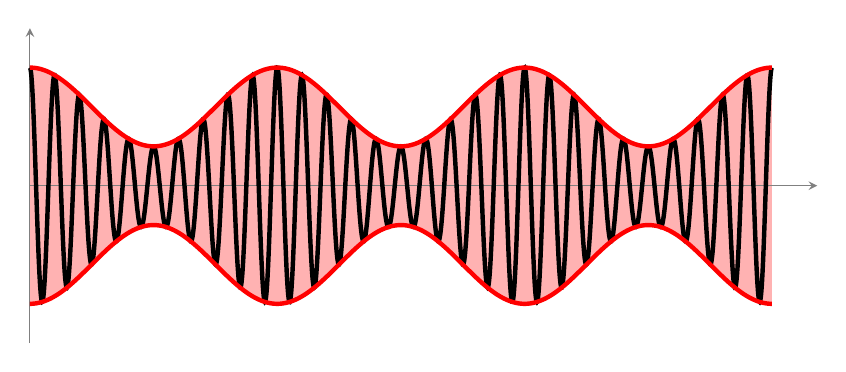
\begin{tikzpicture}[scale=0.5,samples=2000]
	\shade[top color=red,bottom color=red,opacity=0.3] (0,0) -- plot[domain=0:6*pi] (\x,{cos((\x) r)+2}) -- (6*pi,0) -- cycle;
	\shade[top color=red,bottom color=red,opacity=0.3] (0,0) -- plot[domain=0:6*pi,samples=100] (\x,{cos((\x+pi) r)-2}) -- (6*pi,0) -- cycle;
	\draw[color=gray,thin,->,>=stealth] (0,0)--(20,0); % l'axe des abscisses
	\draw[color=gray,thin,->,>=stealth] (0,-4)--(0,4); % l'axe des ordonnées
	\draw [ultra thick,domain=0:6*pi] plot (\x,{2*(1+0.5*cos(\x r))*cos(10*\x r)});
	\draw [color=red,ultra thick,domain=0:6*pi] plot (\x,{cos((\x) r)+2}) plot (\x,{cos((\x+pi) r)-2});
	\end{tikzpicture}
	\end{center}
	\caption{Modulation d'amplitude (AM ou A3E)}
	\end{figure}
	
	NB : à l'examen, ce type de modulation est souvent représenté non pas avec une courbe, mais avec une ligne brisée pour représenter l'enveloppe. Cela donne à peu prés ceci (éventuellement, l'enveloppe peut ne pas être régulière).
	
	\begin{figure}[H]
	\begin{center}
	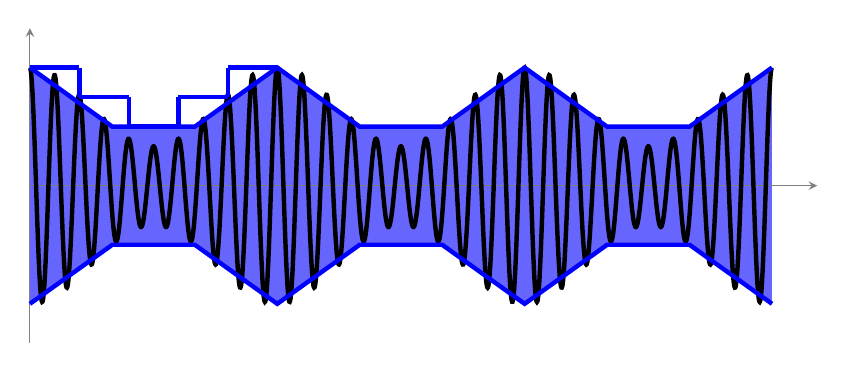
\begin{tikzpicture}[scale=0.5]
	\shade[top color=blue,bottom color=blue,opacity=0.6] (0,0) -- plot[domain=0:6*pi,samples=10] (\x,{cos((\x) r)+2}) -- (6*pi,0) -- cycle;
	\shade[top color=blue,bottom color=blue,opacity=0.6] (0,0) -- plot[domain=0:6*pi,samples=10] (\x,{cos((\x+pi) r)-2}) -- (6*pi,0) -- cycle;
	\draw[color=gray,thin,->,>=stealth] (0,0)--(20,0); % l'axe des abscisses
	\draw[color=gray,thin,->,>=stealth] (0,-4)--(0,4); % l'axe des ordonnées
	\draw [ultra thick,domain=0:6*pi,samples=2000] plot (\x,{2*(1+0.5*cos(\x r))*cos(10*\x r)});
	\draw [color=blue,ultra thick,domain=0:6*pi,samples=10] plot (\x,{cos((\x) r)+2}) plot (\x,{cos((\x+pi) r)-2});
	\draw [color=blue,ultra thick](0,3) -- (1*2*pi/5,3);
	\draw [color=blue,ultra thick](1*2*pi/5,3) -- (1*2*pi/5,2.25);
	\draw [color=blue,ultra thick](1*2*pi/5,2.25) -- (2*2*pi/5,2.25);
	\draw [color=blue,ultra thick](2*2*pi/5,2.25) -- (2*2*pi/5,1.5);
	\draw [color=blue,ultra thick](2*2*pi/5,1.5) -- (3*2*pi/5,1.5);
	\draw [color=blue,ultra thick](3*2*pi/5,1.5) -- (3*2*pi/5,2.25);
	\draw [color=blue,ultra thick](3*2*pi/5,2.25) -- (4*2*pi/5,2.25);
	\draw [color=blue,ultra thick](4*2*pi/5,2.25) -- (4*2*pi/5,3);
	\draw [color=blue,ultra thick](4*2*pi/5,3) -- (5*2*pi/5,3);
	\end{tikzpicture}
	\end{center}
	\caption{Modulation d'amplitude (AM ou A3E)}
	\end{figure}
	
	\begin{figure}[H]
	\begin{center}
	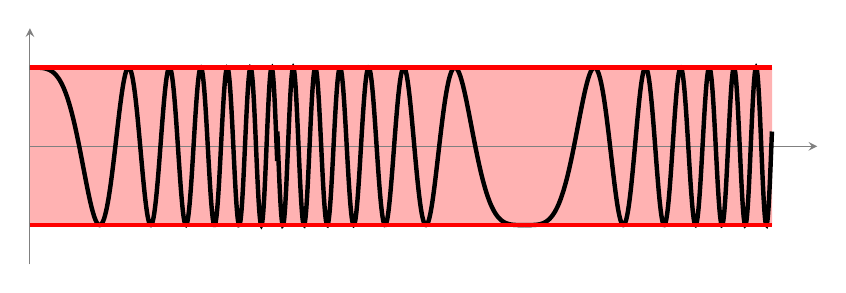
\begin{tikzpicture}[scale=0.5,samples=500]
	\shade[top color=red,bottom color=red,opacity=0.3] (0,2) -- (6*pi,2) -- (6*pi,-2) -- (0,-2);
	\draw[color=gray,thin,->,>=stealth] (0,0)--(20,0); % l'axe des abscisses
	\draw[color=gray,thin,->,>=stealth] (0,-3)--(0,3); % l'axe des ordonnées
	\draw [ultra thick,domain=0:2*pi] plot (\x,{2*(cos((\x*\x) r))});
	\draw [ultra thick,domain=2*pi:4*pi,rotate=180,xshift=-18.85cm] plot (\x,{2*(cos((\x-2*pi)*(\x-2*pi) r))});
	\draw [ultra thick,domain=4*pi:6*pi] plot (\x,{-2*(cos((\x-4*pi)*(\x-4*pi) r))});
	\draw [color=red,ultra thick,domain=0:6*pi] plot (\x,{2}) plot (\x,{-2});
	\end{tikzpicture}
	\end{center}
	\caption{Modulation de fréquence (FM ou F3E) ou modulation de phase (G3E)}
	\end{figure}
	
	\begin{figure}[H]
	\begin{center}
	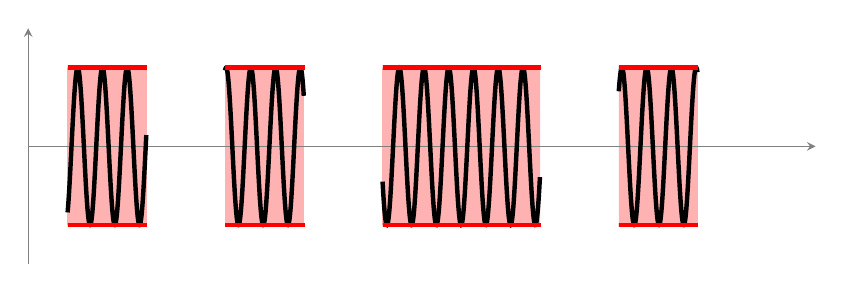
\begin{tikzpicture}[scale=0.5,samples=500]
	\shade[top color=red,bottom color=red,opacity=0.3] (1,2) -- (3,2) -- (3,-2) -- (1,-2);
	\shade[top color=red,bottom color=red,opacity=0.3] (5,2) -- (7,2) -- (7,-2) -- (5,-2);
	\shade[top color=red,bottom color=red,opacity=0.3] (9,2) -- (13,2) -- (13,-2) -- (9,-2);
	\shade[top color=red,bottom color=red,opacity=0.3] (15,2) -- (17,2) -- (17,-2) -- (15,-2);
	\draw[color=gray,thin,->,>=stealth] (0,0)--(20,0); % l'axe des abscisses
	\draw[color=gray,thin,->,>=stealth] (0,-3)--(0,3); % l'axe des ordonnées
	\draw [ultra thick,domain=1:3] plot (\x,{2*(cos((10*\x) r))});
	\draw [ultra thick,domain=5:7] plot (\x,{2*(cos((10*\x) r))});
	\draw [ultra thick,domain=9:13] plot (\x,{2*(cos((10*\x) r))});
	\draw [ultra thick,domain=15:17] plot (\x,{2*(cos((10*\x) r))});
	\draw [color=red,ultra thick,domain=1:3] plot (\x,{2}) plot (\x,{-2});
	\draw [color=red,ultra thick,domain=5:7] plot (\x,{2}) plot (\x,{-2});
	\draw [color=red,ultra thick,domain=9:13] plot (\x,{2}) plot (\x,{-2});
	\draw [color=red,ultra thick,domain=15:17] plot (\x,{2}) plot (\x,{-2});
	\end{tikzpicture}
	\end{center}
	\caption{Tout ou rien (CW ou A1A)}
	\end{figure}	
